%
% File acl2020.tex
%
%% Based on the style files for ACL 2020, which were
%% Based on the style files for ACL 2018, NAACL 2018/19, which were
%% Based on the style files for ACL-2015, with some improvements
%%  taken from the NAACL-2016 style
%% Based on the style files for ACL-2014, which were, in turn,
%% based on ACL-2013, ACL-2012, ACL-2011, ACL-2010, ACL-IJCNLP-2009,
%% EACL-2009, IJCNLP-2008...
%% Based on the style files for EACL 2006 by 
%%e.agirre@ehu.es or Sergi.Balari@uab.es
%% and that of ACL 08 by Joakim Nivre and Noah Smith

\documentclass[11pt,a4paper]{article}
\usepackage[hyperref]{acl2020}
\usepackage{times}
\usepackage{latexsym}
\renewcommand{\UrlFont}{\ttfamily\small}

% This is not strictly necessary, and may be commented out,
% but it will improve the layout of the manuscript,
% and will typically save some space.
\usepackage{microtype}
\usepackage{graphicx}
\graphicspath{ {images/} }
\raggedbottom
\usepackage{colortbl}
\usepackage{color}
\usepackage{booktabs}
\newcommand{\Secref}[1]{Section~\ref{#1}} 

\aclfinalcopy % Uncomment this line for the final submission
%\def\aclpaperid{***} %  Enter the acl Paper ID here

%\setlength\titlebox{5cm}
% You can expand the titlebox if you need extra space
% to show all the authors. Please do not make the titlebox
% smaller than 5cm (the original size); we will check this
% in the camera-ready version and ask you to change it back.

\newcommand\BibTeX{B\textsc{ib}\TeX}

\title{Evaluating the Efficacy of Attention Mechanisms on the Captioning of Images Taken by Visually Impaired People}

\author{Catherine Viloria \\
  University of Gothenburg \\ 
  \texttt{gusviloca@student.gu.se}}

\date{}

\begin{document}
\maketitle
\begin{abstract}
yaaa
\end{abstract}

\section{Introduction}

Image caption generation continues to be a pertinent task within both the computer vision community and the natural language processing (NLP) research field. However, it is important for researchers to also consider how advancements in this field can and will affect users in the real world. Developing models that will be able to effectively and efficiently assist visually impaired users in their day-to-day lives is a challenge in the field to this day. Models that are considered to have a high performance in automatically generating captions will not necessarily perform well in a domain-specific task. Captions for the visually impaired must be detailed yet concise and prioritise the objects of interest within the image. Another factor that could affect a model’s performance would be the quality of the images that are typically associated with caption generation for this task. It is not uncommon for images to be in the wrong orientation, unfocused, and out of frame. While any improvement in image captioning is still a step forward, critically examining applications of these models in situations that are not as contrived is extremely important. 

In this project, the VizWiz dataset presented by \citet{Gurari-2020-captioning}, specifically created to represent the blind and visually impaired community, is used to train an encoder-decoder model with attention to examine how a standard image captioning model will perform in generating captions for the visually impaired. Evaluating the neural image caption generator with visual attention presented by \citet{Xu-2015-show-attend} through a domain-specific lens is important for the community being affected but also will have research-related contributions. Choosing to assess a model in this way presents nuances that are sometimes overlooked when implementing these models. It will also shed light on how humans would approach a task and eventually the possibility of replicating said modus operandi or intuition in a model. The problem of the gap between the two modalities—image and text—presented in \citet{Bernardi-2016-automatic} is also discussed. The extent of how bad this problem will be in this model is shown to be exacerbated because of the dataset used since grounding becomes an even more difficult task. 

The following sections are organised as follows. Section 2 introduces image caption generation and the models and attention mechanism that precede what was implemented for this paper. In Section 3, the VizWiz dataset and specifics of the model implementation are given. The results are presented in Section 4. Section 5 discusses the results. Specific plans for future work are defined in Section 6 and it is followed by the conclusion and future work in Section 7. References are provided in Section 8.

\section{Related Work}
Automatic description generation from images has been a challenging task that both the computer vision and natural language processing communities have taken an interest in. \citet{Bernardi-2016-automatic} surveys the current approaches to this task and classifies these approaches through how they conceptualise the problem—either a generation problem, a retrieval from a visual space problem, or a retrieval from a multimodal space problem. All three approaches have their advantages and disadvantages. The first two approaches choose to rely more heavily on one modality (visual or textual) to base the predictions for generating captions while the third approach attempts to combine both representations to make the final image description. The implementation in this paper is the third approach. This approach attempts to address the semantic gap or mapping problem between language and image representations through the attentional component. The attention mechanism allows us to see visualizations of which regions in an image are salient and where the model is “looking” when generating each word in the caption.

The model implemented in this paper is a combination of proposed methods from two different, but related, research areas—image captioning and machine translation. \citet{Vinyals-2014-showandtell}’s seminal paper \emph{Show and Tell} presents a neural image caption generator (NIC) that uses a vision convolutional neural network (CNN) that encodes images with richer representations to a fixed dimension for the decoder. The encoder’s output is then passed to a language-generating recurrent neural network (RNN)—an LSTM-based sentence generator. Their model demonstrates that this approach significantly improves both accuracy and fluency when generating captions. A neural machine translation with an attention mechanism is proposed in \citet{Bahdanau-2014-neural}. Attention allows the model to look for parts in the source sentence that would be most relevant in predicting the target word. The flexibility of alignment between the source and target sentences introduced through attention allows for better translations, especially between languages that have syntactical differences. 

The combination of NIC and an attention mechanism resulted in the model implemented by \citet{Xu-2015-show-attend}—a neural image caption generator with visual attention. The encoder uses low-level representations which prioritises salient features of an image. The attention component adds “an extra layer of interpretability to the output of the model” \citep{Xu-2015-show-attend} and the alignments learned by the model correspond very well with human intuition. The motivations and intuitions of choosing to use the model implemented by \citet{Xu-2015-show-attend} for this domain-specific task is discussed in Section 3. 


\section{Dataset \& Methodology}
\subsection{VizWiz Dataset}
The domain-specific dataset used for this project was the VizWiz dataset \footnote{\url{https://vizwiz.org/}}. It is comprised of 39,181 images taken by people who are either blind or visually impaired. The images of the dataset come from a mobile phone application made to support real-world users through their visual description service. Users take a picture, record a spoken question and are then connected with people that could assist them. The VizWiz dataset has also been developed for various computer vision tasks, all related and extremely useful for the visually impaired community: image captioning, image quality assessment, visual question answering (VQA), answer-difference reasoning, vision skills for VQA, and visual privacy recognition. The VizWiz dataset is “a valuable foundation for designing more generalized computer vision algorithms that meet the large diversity of needs for real end users” \citep{Gurari-2020-captioning}. 

\subsubsection{VizWiz-Captions Dataset}
For this project, the VizWiz-Captions dataset \footnote{\url{https://vizwiz.org/tasks-and-datasets/image-captioning/}} was used. Each image is paired with 5 human-made captions collected through crowdsourcing via Amazon Mechanical Turk. Due to GPU limitations and consciousness of memory usage, only the training dataset was used. The training dataset originally had 23,141 images and 117,155 captions. After examining some of the metadata included in the dataset, a filtering process was conducted. If an image was considered to be spam (\emph{is\_rejected} column) or considered to have quality issues by annotators (\emph{is\_precanned} column, if True had “Quality issues are too severe to recognize visual content.” as its caption), they were filtered out of the dataset. Images with the characteristic of having text were kept since text is one of the main reasons why someone who is visually impaired would need assistance. After filtering, there were 14,790 images left and the model implementation was done with a 60/20/20 train, validation, test split (8,874 train, 2,958 validation, and 2,958 test).

\subsubsection{Annotator Reliability \& Ethical Considerations}
Although it is incredibly important to collect human-made captions for any text generation task, the process and its output also present some challenges and factors that must be considered. While it is greatly advantageous for a model to learn from human-made captions, humans are not perfect and also make mistakes. Crowdsourcing allows researchers to reach a larger, more widespread and diverse demographic but it also makes it much more difficult to oversee and guide annotators to ensure that the captions being made are of the best quality. The instructions provided to annotators presented in \citet{Gurari-2020-captioning}, while understandably so given the conditions of the annotation process, were very concise and left space for restrictions on the annotators that would affect the dataset and future model implementations.  

Examples of instructions that could lead to problems when training models are: “Include at least eight words.”, “Describe all parts of the image that may be important to a person who is blind.”, and “If text is in the image, and is important, then you can summarize what it says. DO NOT use all the specific phrases that you see in the image as your description of the image.” \citep{Gurari-2020-captioning} If an annotator was able to effectively describe an image with 4 words (e.g. “Can of mushroom soup.”), they are then required to add additional information that might not be neither useful nor necessary. The second instruction can also be interpreted as subjective and what one annotator thinks is useful information for a person who is blind, another annotator might not think similarly. Finally, the third instruction requiring a summarization of text that appears in an image rather than providing a word-for-word description makes it extremely difficult to ground any generated caption for a model. Although text summarization would be useful for this real-world task, it is a completely different task that is overlooked when training an image caption generator. 

Since annotators were also found through crowdsourcing, annotator reliability could possibly be a point of contention. Not only are the annotators’ backgrounds unknown, they are also inconsistent. In an ideal world, it would have been better to have real-world users with high ratings of the mobile application to come in and annotate images as they have domain-specific knowledge and skills. Ethical concerns may also affect the quality of work annotators submit. It is extremely important to acknowledge the absolutely dismal wages provided to annotators through Amazon Mechanical Turk.\citep{hara2018amazon} The low wages and absence of work benefits can also affect the care and quality of the captions made by annotators. With these considerations, an example is provided in \autoref{fig:vwcaption} of how varied and inconsistent the quality and structure of captions can be within the dataset. The variation in complexity and length is quite large and can be argued to be either advantageous or disadvantageous for a model when training. 

\begin{figure}[h]
  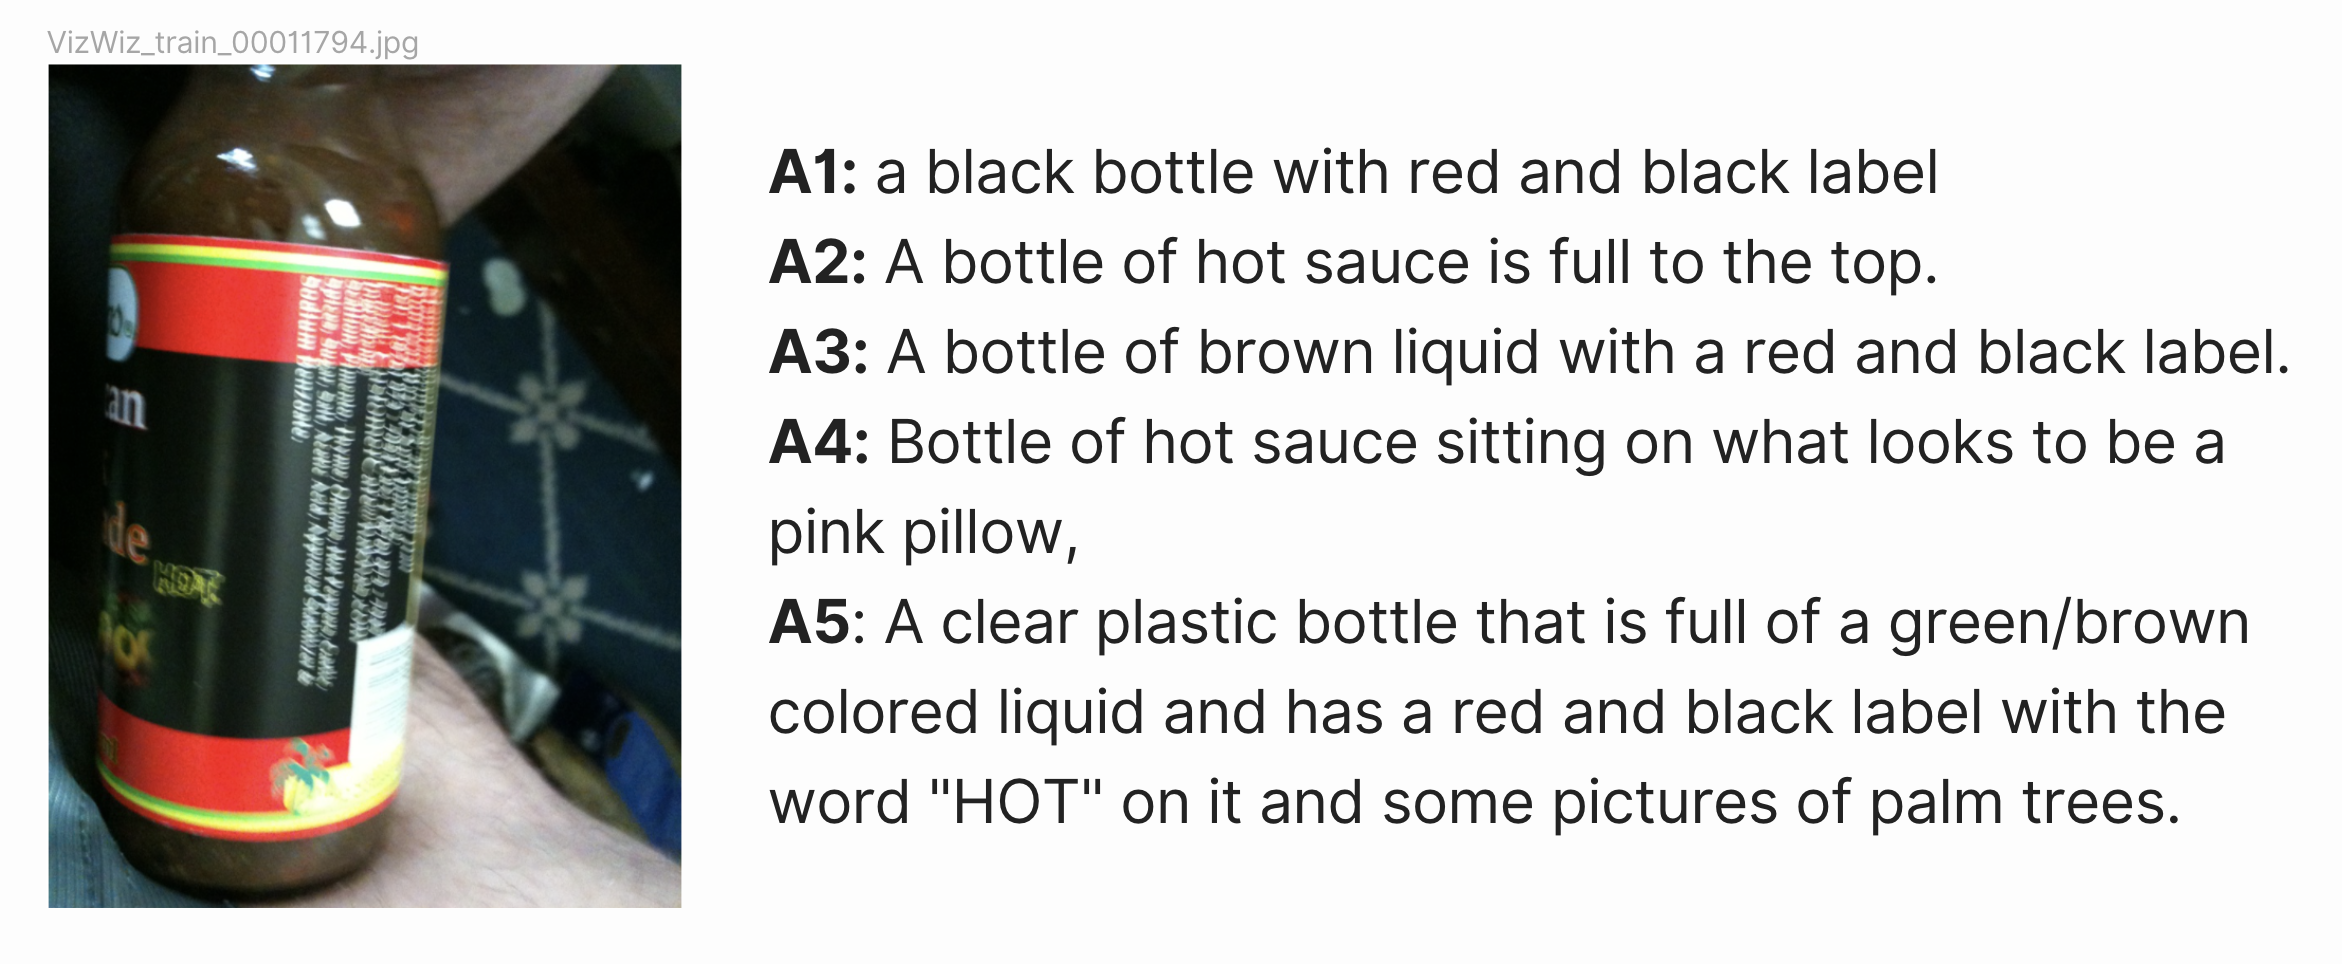
\includegraphics[width=\linewidth]{VizWiz_train_00011794_captioned.png}
  \caption{An image from the VizWiz-Captions dataset and 5 captions from 5 different annotators.}
  \label{fig:vwcaption}
\end{figure}

\subsection{Model Architecture}
The model implemented was an encoder-decoder with an attention mechanism. The PyTorch Tutorial to Image Captioning by Sagar Vinodababu\footnote{\url{https://github.com/sgrvinod/a-PyTorch-Tutorial-to-Image-Captioning#training}} was followed and the implementation included an encoder that was pretrained on ResNet. The encoder is responsible for taking the images as input and transforming it into smaller representations. It returns a “state” that is fed into the decoder. The decoder is then responsible for interpreting the output of the encoder. It also calculates the attention weights for the image. (*also generates caption/ language model??)

Creating low-level representations when passed through the encoder seemed like a good approach for this task since a lot of images in the dataset only have one object as the focal point and this object is only partially shown in the image. A lower-level representation or a representation that is closer to what the image actually looks like would be very helpful rather than having a representation that is an average of everything in the picture. This approach would be called the top-down approach—contrasted with the bottom-up approach which is good for semantically-rich images where multiple objects within the image are first identified and then given to the encoder. \citep{Anderson-2017-bottomuptopdown} Datasets that have high-quality and semantically-rich images, such as MSCOCO, are more ideal for the top-down approach.

During training, sequences are padded then ordered by length in order to minimise computations (****???wording). Word embeddings, attention weights, and the decoder all have a dimension of 512 with a batch size of 32. The encoder’s learning rate was 0.0001 and the decoder’s learning rate was 0.0004. Early stopping was implemented after 20 epochs of no improvement. These hyperparameters and implementations were all chosen through the tutorial source.  

The greedy search algorithm was implemented for generating captions. In the greedy search algorithm, when given a number of choices in the next stage, the model will always choose the best immediate output. For this task, the language model takes the vocabulary’s logits and turns them into probabilities. This is then fed to the greedy search algorithm where it chooses the highest probable word to occur next at each stage. However, greedy search also has its drawbacks. Since it only chooses the best immediate output and does not look farther ahead, it has a higher chance of not reaching the globally optimum solution—hence its name, \emph{greedy} search.

\section{Results}
\label{sec:results}

Upon initial review, results were abysmal but with further examination and analysis, lessons were learned. In this section, results will be presented and their causes will also be explained. The sections following will include the extrapolations of the results and the conclusions that come with them. 

The corpus-BLEU score was used as the main measure for this project which requires a list of references (the human-made annotations) and a candidate (the predicted caption). It is the average of the scores between the candidate and each reference. Both sentence BLEU and corpus BLEU calculate the cumulative 4-gram BLEU score (BLEU-4) by default. Although a great option to calculate scores for a task that has more than one caption, longer sentences also lead to lower scores. Since the variation of lengths, even with a minimum of 8 words per caption, are quite large, this task will still be affected as seen on \autoref{tab:bctest}. Detailed captions are also valued for this task. However, the detail provided by annotators are often distinctive to the individual as annotators were encouraged to summarise texts and decide what in the image they think might be important for a blind person.

%---table: bc test---
\begin{table}[h]
\centering
\begin{tabular}{llll} 
\toprule
 & \textbf{Loss} & \textbf{Accuracy} & \textbf{BLEU-4} \\ 
\hline
\textit{BC} & 4.114 & 64.060 & 0.142178 \\
TEST & 4.181 & 63.941 & 0.145776 \\
\bottomrule
\end{tabular}
\vspace{2mm}
\caption{\label{tab:bctest}Loss, Top-5 Accuracy, and BLEU-4 scores for the best performing model (BC for best checkpoint) during training and testing.}
\end{table}
%--- end of table

The training process also included a mechanism that saves and labels the best performing model as a checkpoint which will be used for validation and testing. \autoref{fig:lossgraph} and \autoref{fig:accuracygraph} show the loss and accuracy curves during training. The blue circle marker indicates the model used for validation and testing. In both curves, there are clearly other epochs where the model’s loss was lower, and the accuracy was higher. However, the model chosen to proceed with was decided through the highest BLEU-4 score. This can also be seen in \autoref{trainingdata} where the highest accuracy was attained on epoch 12 while the highest BLEU-4 score was attained on epoch 14. 

% loss graph figure
\begin{figure}[h]
  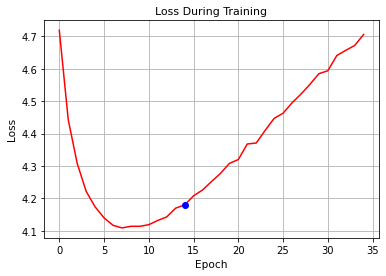
\includegraphics[width=\linewidth]{paper/images/loss_graph.png}
  \caption{Loss curve during training. The blue point is the loss for the best performing model model based on its BLEU-4 score.}
  \label{fig:lossgraph}
\end{figure}
% ----end of figure----

% accuracy graph figure
\begin{figure}[h]
  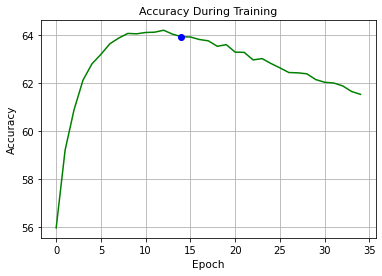
\includegraphics[width=\linewidth]{paper/images/accuracy_graph.png}
  \caption{Accuracy curve during training. The blue point is the accuracy for the best performing model based on its BLEU-4 score.}
  \label{fig:accuracygraph}
\end{figure}
% ----end of figure----

% training stats table
\begin{table}
\centering
\begin{tabular}{|c|c|c|} 
\hline
\rowcolor[rgb]{0.761,0.761,0.761} \textbf{Epochs} & \textbf{Top-5 Accuracy} & \textbf{BLEU-4}  \\ 
\hline
0                                                 & 55.982                  & 0.1047           \\ 
\hline
1                                                 & 59.216                  & 0.1180           \\ 
\hline
2                                                 & 60.894                  & 0.1277           \\ 
\hline
3                                                 & 62.122                  & 0.1307           \\ 
\hline
4                                                 & 62.798                  & 0.1362           \\ 
\hline
5                                                 & 63.192                  & 0.1371           \\ 
\hline
6                                                 & 63.632                  & 0.1404           \\ 
\hline
7                                                 & 63.87                   & 0.1429           \\ 
\hline
8                                                 & 64.06                   & 0.1421           \\ 
\hline
9                                                 & 64.045                  & 0.1440           \\ 
\hline
10                                                & 64.1                    & 0.1447           \\ 
\hline
11                                                & 64.112                  & 0.1449           \\ 
\hline
12                                                & \textbf{64.193}         & 0.1451           \\ 
\hline
13                                                & 64.031                  & 0.1445           \\ 
\hline
\rowcolor[rgb]{0.992,0.992,0.588} 14              & 63.923                  & \textbf{0.1465}  \\ 
\hline
15                                                & 63.912                  & 0.1461           \\ 
\hline
16                                                & 63.808                  & 0.1460           \\ 
\hline
17                                                & 63.753                  & 0.1459           \\ 
\hline
18                                                & 63.526                  & 0.1456           \\ 
\hline
19                                                & 63.594                  & 0.1452           \\ 
\hline
20                                                & 63.283                  & 0.1427           \\ 
\hline
21                                                & 63.275                  & 0.1429           \\ 
\hline
22                                                & 62.96                   & 0.1434           \\ 
\hline
23                                                & 63.015                  & 0.1421           \\ 
\hline
24                                                & 62.811                  & 0.1422           \\ 
\hline
25                                                & 62.629                  & 0.1419           \\ 
\hline
26                                                & 62.436                  & 0.1423           \\ 
\hline
27                                                & 62.424                  & 0.1416           \\ 
\hline
28                                                & 62.383                  & 0.1400           \\ 
\hline
29                                                & 62.144                  & 0.1383           \\ 
\hline
30                                                & 62.031                  & 0.1403           \\ 
\hline
31                                                & 62.002                  & 0.1382           \\ 
\hline
32                                                & 61.882                  & 0.1389           \\ 
\hline
33                                                & 61.649                  & 0.1370           \\ 
\hline
34                                                & 61.53                   & 0.1383           \\
\hline
\end{tabular}
\caption{\label{trainingdata}Top-5 accuracy and BLEU-4 score after each epoch during training. The row highlighted in yellow is the model that performed the best and what was used for validation and testing.}
\end{table}
% ------end of table------

The BLEU-4 score was incredibly low since the captions being generated by the model did not match any of the human-made caption. Since it is difficult to also trust such varied human-made captions as the gold-standard, a manual inspection of the generated captions was done. Below are some examples of what majority of the generated captions looked like:
% examples of captions
\begin{quote}
  ``white background''
\end{quote}
\begin{quote}
  ``a close up of a white background with a black background''
\end{quote}
\begin{quote}
  ``a close up of a black background with a white background with a white background''
\end{quote}
\begin{quote}
  ``a close up of a black background with black lettering''
\end{quote}
\begin{quote}
  ``the photo is cropped out of the frame''
\end{quote}

The captions seem to be recursive and only use words and phrases that refer to the image’s background, alternating from \emph{black} and \emph{white}. These captions are a result of the greedy search algorithm since a large amount of the human-made captions had these phrases at the end of the captions.
	
In evaluating the attention in \autoref{fig:stapler}, \autoref{fig:whitetext}, \autoref{fig:blackscreen}, there seems to be a pattern in where the model is looking while generating captions. The model begins by looking at the entire image, then attends to the middle of the image, typically in the top right and makes its way to the bottom left. The purpose of visualizing attention is not being achieved and these visualizations do not connect nor ground the captions it has generated for their respective images. 

% attention - stapler
\begin{figure}[ht]
  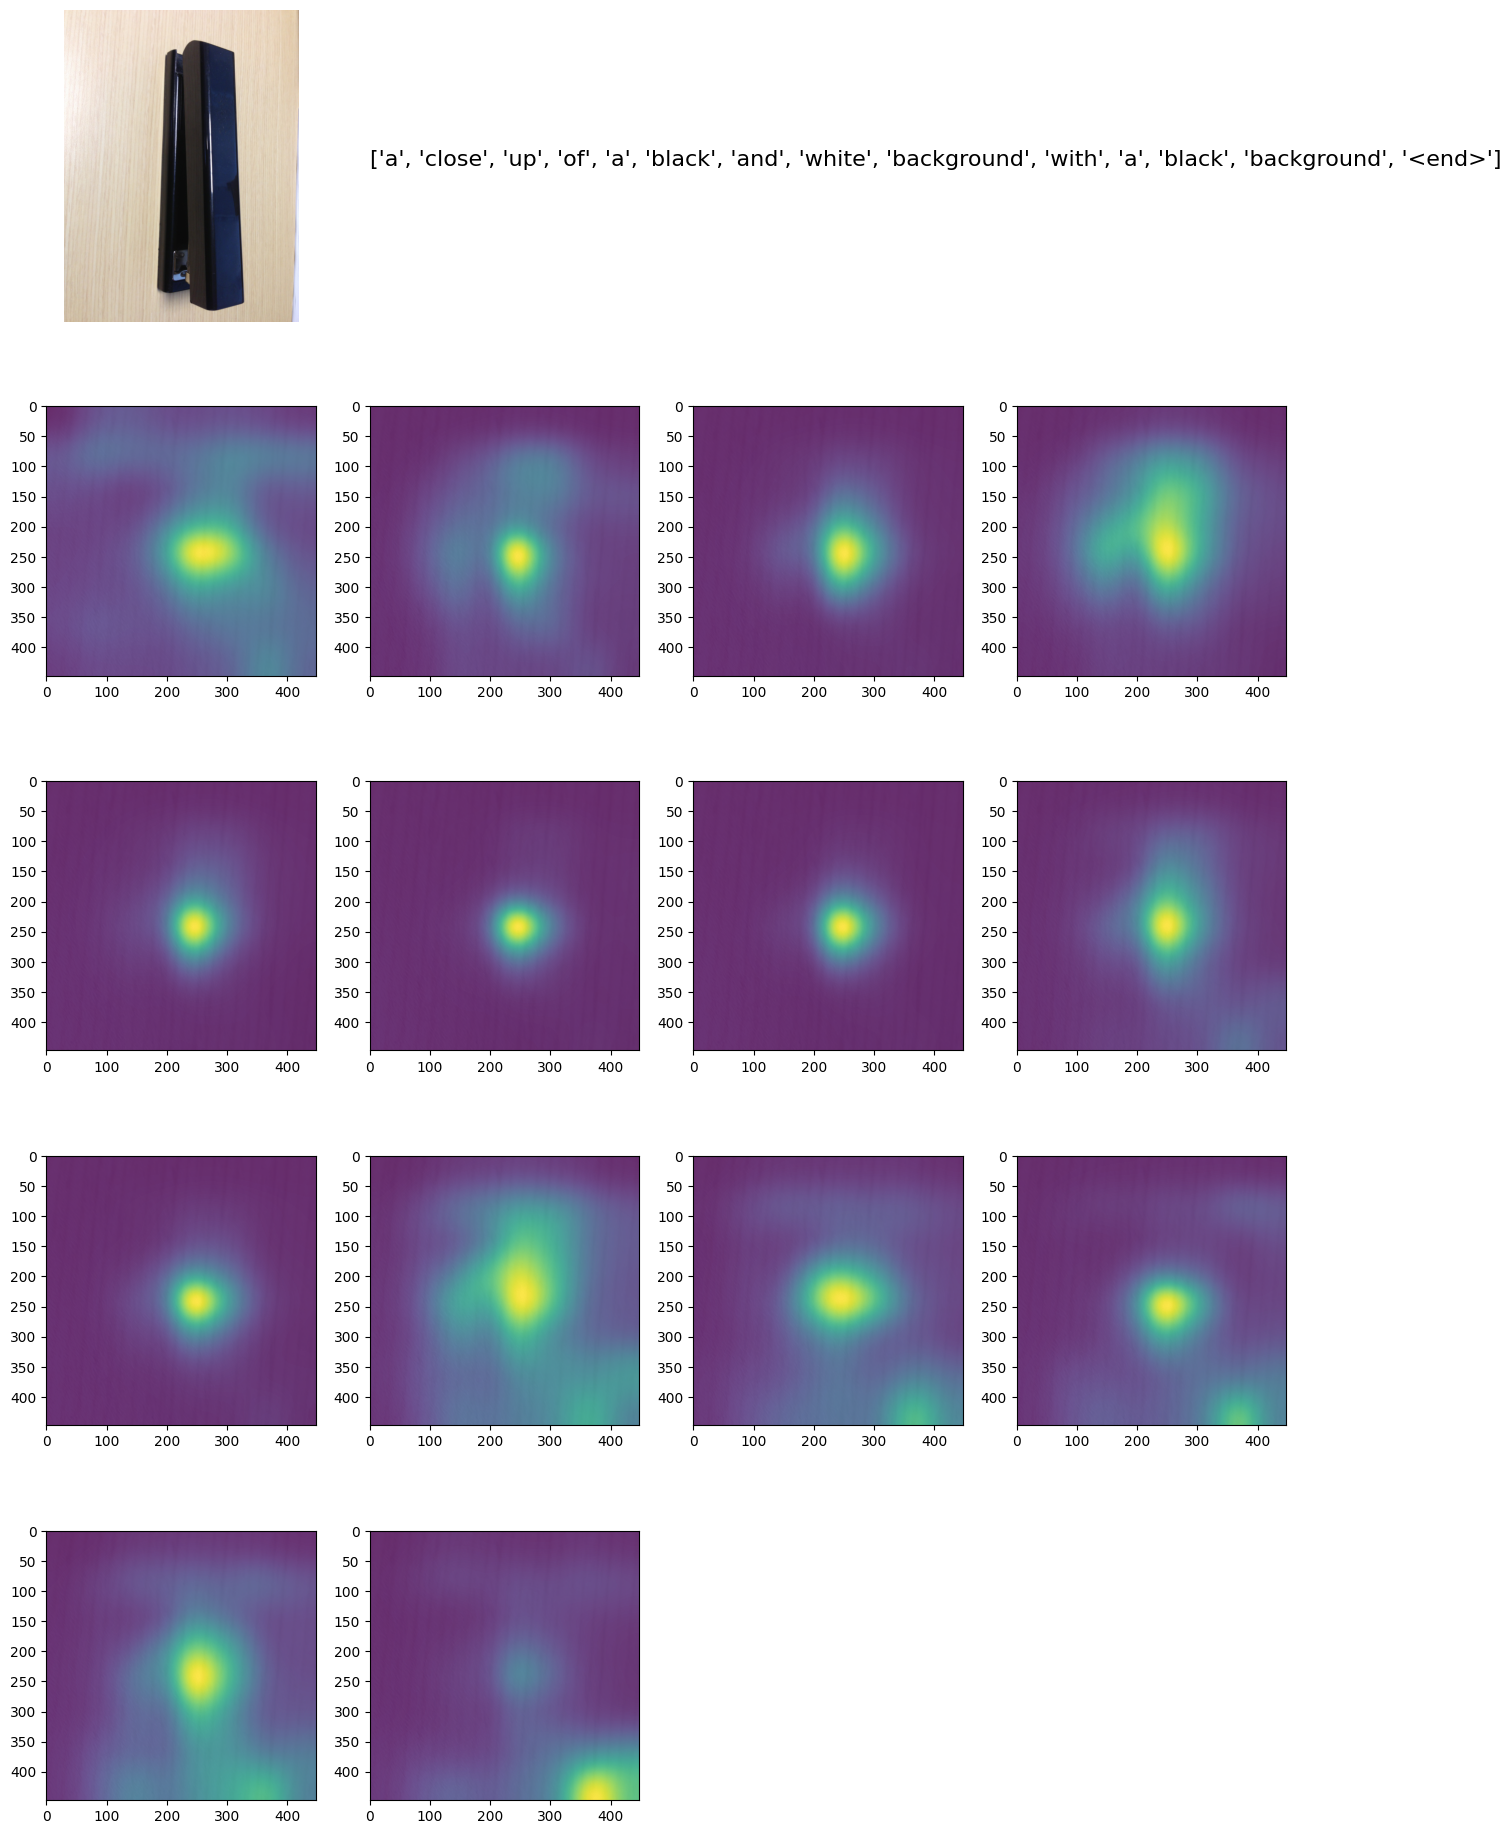
\includegraphics[width=\linewidth]{VizWiz_train_00013366.png}
  \caption{Attention visualized for captioning an image of a stapler in the wrong orientation (portrait instead of landscape)(VizWiz\_train\_00013366.png).}
  \label{fig:stapler}
\end{figure}
% ----end of figure----

% attention - whitetext
\begin{figure}[ht]
  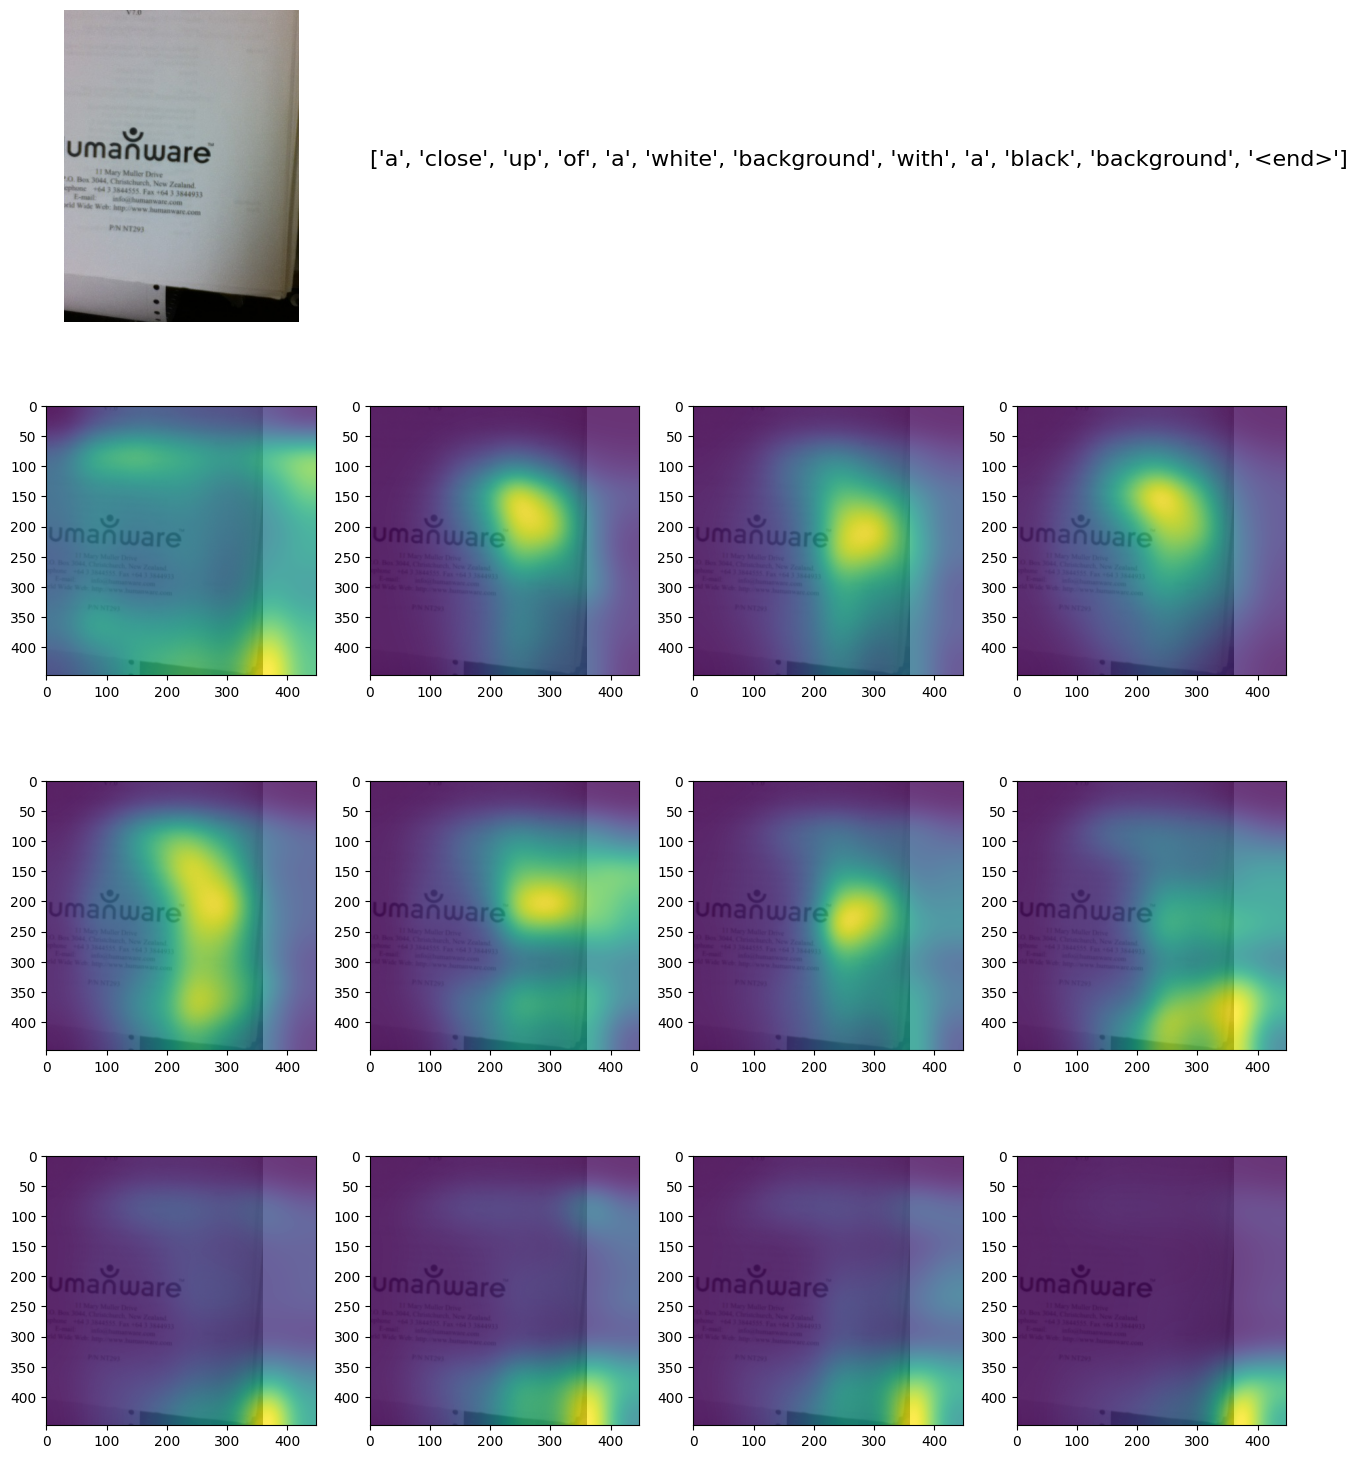
\includegraphics[width=\linewidth]{VizWiz_train_00023423.png}
  \caption{Attention visualized for captioning an image of a white page with text (VizWiz\_train\_00023423.png).}
  \label{fig:whitetext}
\end{figure}
% ----end of figure----

% attention - black screen
\begin{figure}[ht]
  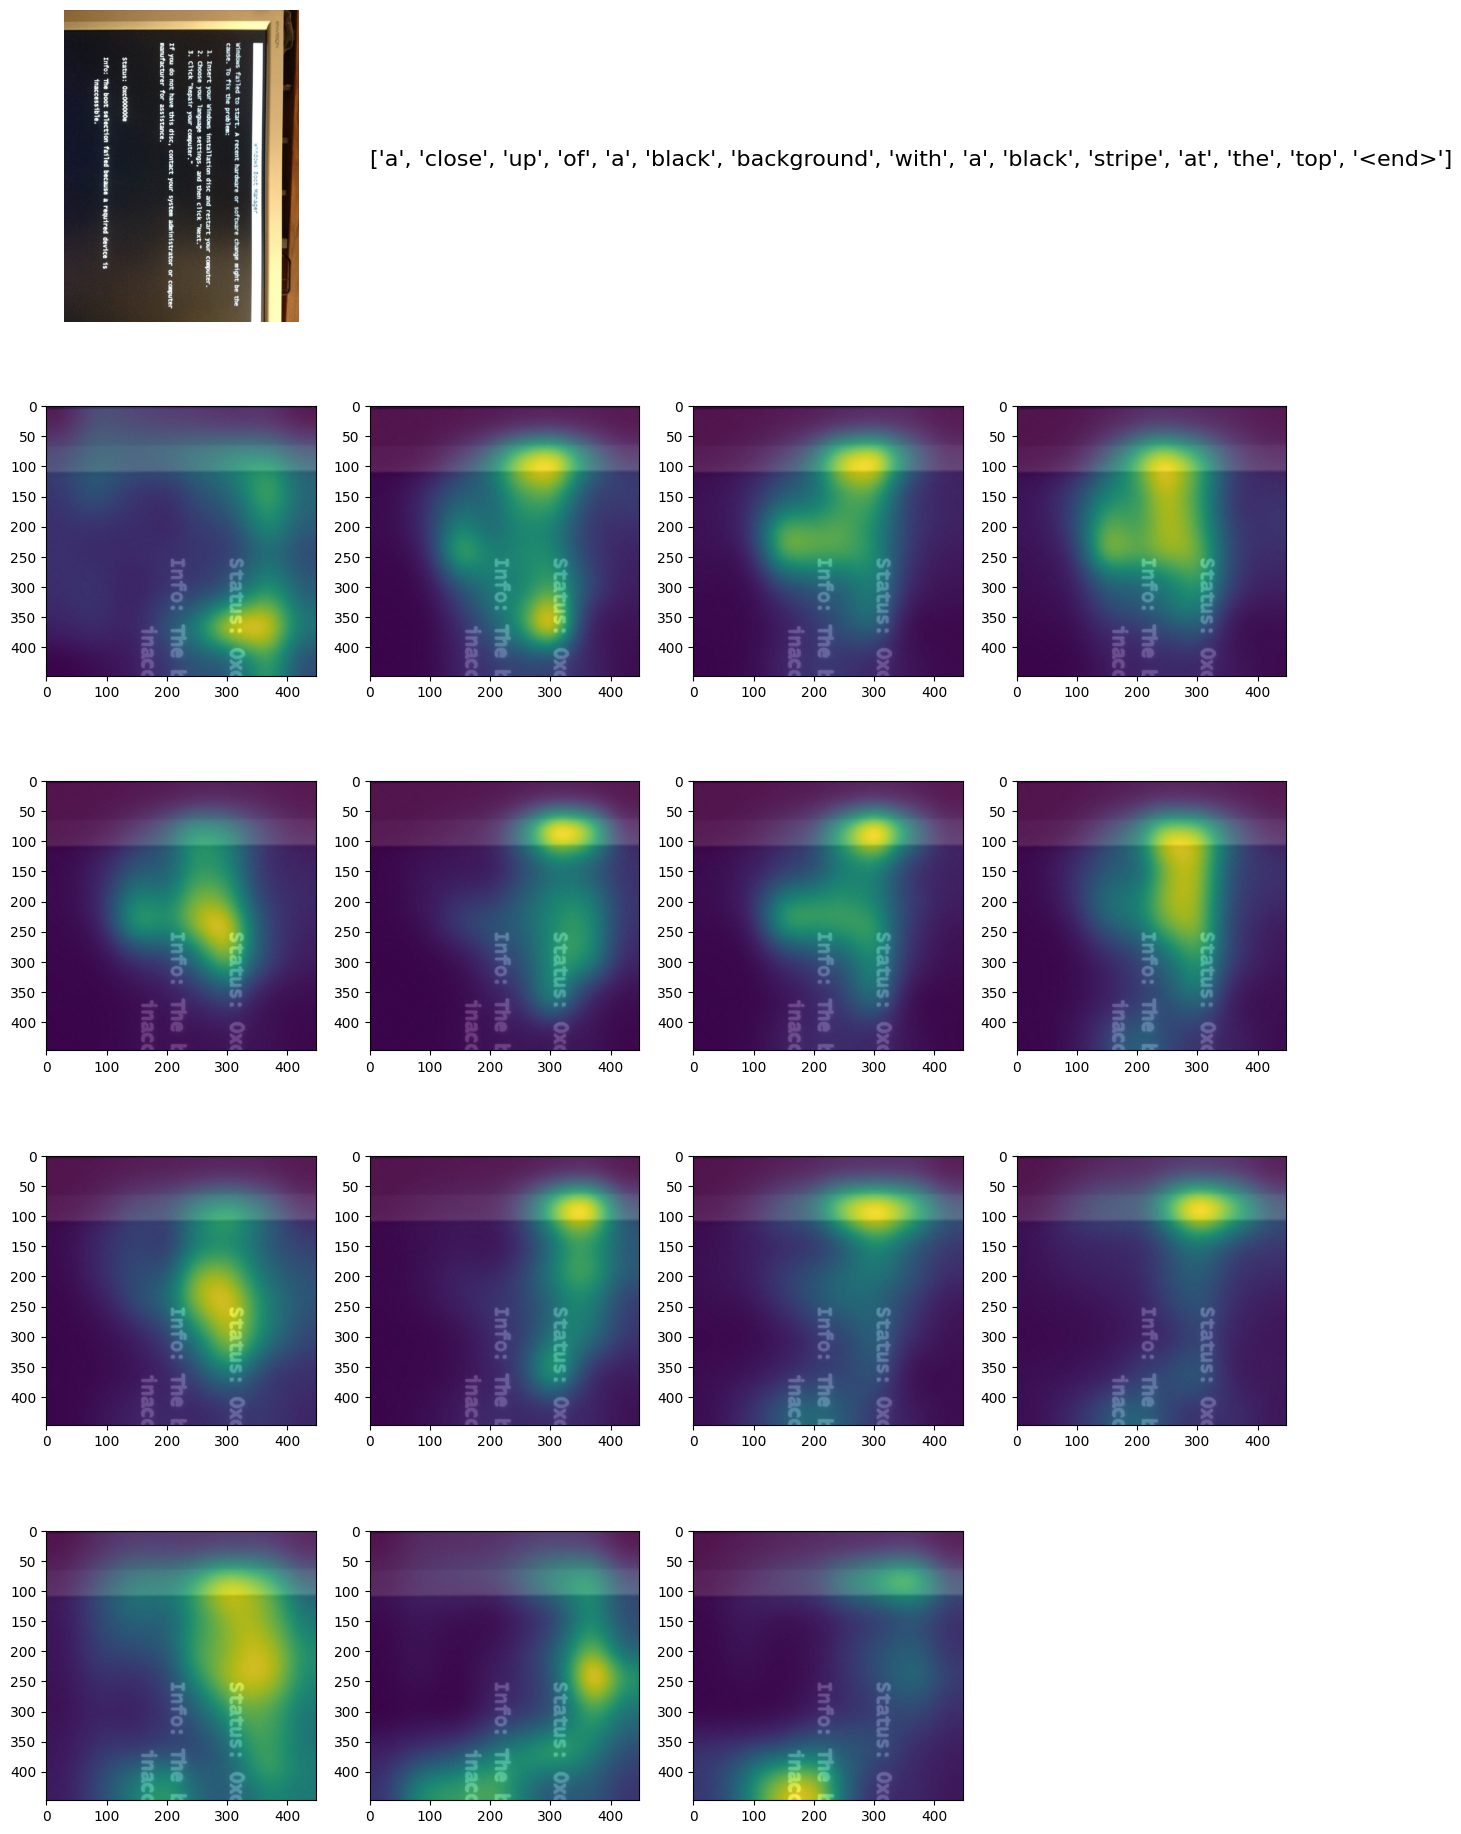
\includegraphics[width=\linewidth]{VizWiz_train_00000858.png}
  \caption{Attention visualized for captioning an image of a black screen with text in the wrong orientation (portrait instead of landscape)(VizWiz\_train\_00000858.png).}
  \label{fig:blackscreen}
\end{figure}
% ----end of figure----

\section{Discussion}
\label{sec:discussion}
Although \citet{Xu-2015-show-attend} presented a state-of-the-art model that performed incredibly well in generating captions for images, this same model being trained on a domain-specific dataset such as VizWiz was unsuccessful. Captions that are considered to be useful for this task does not only require identifying objects in an image. Additionally, acceptable captions can vary in length, style, and wording. There is a lot of space for a caption to be successful despite the specificity and detail it requires. 

The language patterns learned by the model through the human-made captions also seemed to be not useful at all and could be argued to be detrimental. A post-hoc investigation of the human-made captions was done and many annotators seemed to follow a common template for what is deemed to be succinct and effective—begin with describing the foreground and any item that seems to be the focal point, mention any text that appears, describe the background. This kind of template is not ideal for generating captions for images as the words that will often come up in describing text or the background will always be chosen when used with the greedy search algorithm. Once a word with a very high frequency is chosen, the model will continue to choose the common phrase such as “on a white background”. This tendency will turn into a recursive caption like the example given in \Secref{sec:results}, “a close up of a black background with a white background with a white back-ground”. 

There are also data limitations when it comes to the images being fed into the model. Since the photographs were taken and submitted by real-word users, people who are visually-impaired, it should be acknowledged that the images are not of the best quality. Images are described to “often contain text, exhibit a high variability in image quality, and contain a large diversity of content”. \citep{Gurari-2020-captioning} In majority of the images, the object in question is not framed properly and we only have a partial view of said object. Focus of the object or clarity is at times also absent in the images. The importance of interpreting and summarising text for this task also creates an obstacle for a typical image caption generator. There are many characteristics of a photograph that we take for granted when implementing models that generate captions. The difference the orientation of an image should also be taken into consideration. In \autoref{fig:stapler}, a model might identify the object as a stapler if the image was on landscape rather than portrait—the “prototypical” position of a stapler. It is crucial to recognise that images and captions (MSCOCO and Flickr8K) being used to train image caption generators are of high-quality and are quite idyllic compared to the images used to train the model for this project. 

In terms of attention and seeing what the model is looking at while generating the captions, it is a good sign that the attention is quite general in the beginning. However, since the captions are not competent and do not refer to anything in the image, it is not possible to ground the text generated with the image and vice versa—creating a bigger semantic gap. With these results, the question of whether attention is even useful or needed for this task is brought up. Attention was initially added into translation models to account for long dependencies and this transfers for images with many objects. Since this task generally requires a caption that describes the focal point or one object, it might be the case that attention is not actually necessary. Another important consideration is the difficulty of replicating human-made caption. As \citet{miltenburg-pragmatic} states, human-generated image descriptions are rich and subjective. There is “virtually [an] infinite set of different ways to describe an image [and] people will use their own knowledge and expectations to choose from all of those options how an image should be described.” \citep{miltenburg-pragmatic} With an infinite amount of options scattered amongst the captions provided, it is incredibly difficult for a model to learn effective patterns to describe an image like a human would.

\section{Conclusion \& Future Work}
\label{sec:conc&fw}
In this paper, a well-renowned and successful model architecture was implemented with a domain-specific task in mind. Using the VizWiz dataset to represent (replicate? WORD) the real-world use of automated image captioning, the model was incredibly unsuccessful in generating captions considered to be useful for the task at hand. Standard captioning with no pre-training other than the domain-specific task dataset gives a very low performance and training must be done outside of the task dataset and then finetuned. The shortcomings of the greedy search algorithm and overlooked limitations of the dataset also contributed to the bad performance of the model. It is extremely crucial to be critical of the data and how it could influence training—both in improvement and detriment. \citet{miltenburg-pragmatic} states “image description literature has generally avoided these issues by delegating them to the crowd-workers annotating the images.” It is important for both the computer vision and natural language processing communities to consider finding ways to further improve already state-of-the-art models for domain-specific tasks as these would have real-world effects on a very large demographic. The architecture can be questioned as being too simple…or not? There are many more mechanisms that must be implemented in order to account for the components that make this specific task very difficult. However, it could also be said that since the images are much more simpler than typical image captioning photographs, the model should be simpler but given more information. 

\subsection{Future Work}
\label{ssec:futurework}

\subsubsection{Model Architecture}
\label{sssec:modarch}
Alterations to the model architecture would include choosing the beam search algorithm over greedy search since it seems to have caused one of the bigger, more tangible bottlenecks. The beam search algorithm would be more likely to choose the globally optimum solution and deliver more sophisticated and specific captions. The ability to choose the beam size would also allow more flexibility in how far ahead the model should look ahead when making choices at each timestep. Another alteration to consider would be implementing a visual sentinel as \citet{Lu-whentolook} have proposed. This would give the ability to decide whether to rely on the language image or the image through the sentinel gate. This option could give more accurate captions since there will be the chance to prioritise visual information over the word most likely to occur beside the previously chosen word.

\subsubsection{Task-Specific Improvements}
After examining the data further after already having implemented the model and considering the symbiotic relationship between the dataset and model architecture, some task-specific additions might improve the model’s performance. Since there seemed to be a common-template for what is considered to be an effective caption, implementing some sort of rule-based template for the captions first and foremost might help with creating a more realistic and useful caption for the target demographic. Another important consideration is the vital need to read and summarise text in images. Implementing some form of optical character recognition (OCR) and text summarisation would be extremely helpful. A mechanism where if text is detected, it will be used. Additionally, since annotators were instructed to summarise the text rather than repeating what is said, summarising the text output of an OCR mechanism could possibly better mirror the human-made captions in the dataset.

\bibliography{anthology,acl2020}
\bibliographystyle{acl_natbib}

\end{document}
